\begin{enumerate}[label=\thechapter.\arabic*,ref=\thechapter.\theenumi]
\item Let a frequency modulated (FM) signal : $ x(t) = A \cos(\omega_c t + k_f \int_{-\infty}^{t} m(\lambda) d\lambda)$ , where $ m(t) $is a message signal of bandwidth $ W $. It is passed through a non-linear system with output $y(t) = 2x(t) + 5(x(t))^2 $.
Let $B_T $denote the FM bandwidth. The minimum value of $ \omega_c $ required to recover $ x(t) $ from $ y(t) $ is:\\
\begin{enumerate}[label = (\Alph*)]
\item $B_T + W$ \\
\item $\dfrac{3}{2} B_T$ \\
\item $2B_T + W$ \\
\item $\dfrac{5}{2} B_T$ \\
\end{enumerate}

\solution
\newpage

\item Let an input $x[n]$ having discrete-time Fourier transform
$X(e^{j\Omega}) = 1 - e^{-j\Omega} + 2e^{-3j\Omega}$
be passed through an LTI system. The frequency response of the LTI system is 
$H(e^{j\Omega}) = 1 - \frac{1}{2} e^{-2j\Omega}$
The output $y[n]$ of the system is \\ \hfill(GATE EC 2023)
\solution 
\newpage
\item The Fourier transform $X(\omega)$ of $x(t) = e^{-t^2}$ is\\
Note:$\int_{-\infty}^{\infty} e^{-y^2} \,dy = \sqrt{\pi}$ \\  
A) $\sqrt{\pi} e^{\frac{\omega^2}{2}}$ \\
B) $\frac{e^{\frac{-\omega^2}{4}}}{2\sqrt{\pi}}$ \\
C) $\sqrt{\pi} e^{\frac{-\omega^2}{4}}$ \\
D) $\sqrt{\pi} e^{\frac{-\omega^2}{2}}$\\
\hfill Gate 2023 EC Question 28
\solution
\let\negmedspace\undefined
\let\negthickspace\undefined
\documentclass[journal,12pt,twocolumn]{IEEEtran}
\usepackage{cite}
\usepackage{amsmath,amssymb,amsfonts,amsthm}
\usepackage{algorithmic}
\usepackage{graphicx}
\usepackage{textcomp}
\usepackage{xcolor}
\usepackage{txfonts}
\usepackage{listings}
\usepackage{enumitem}
\usepackage{mathtools}
\usepackage{gensymb}
\usepackage{comment}
\usepackage[breaklinks=true]{hyperref}
\usepackage{tkz-euclide} 
\usepackage{listings}                                   
\def\inputGnumericTable{}                                 
\usepackage[latin1]{inputenc}                                
\usepackage{color}                                            
\usepackage{array}                                            
\usepackage{longtable}                                       
\usepackage{calc}                                             
\usepackage{multirow}                                         
\usepackage{hhline}                                           
\usepackage{ifthen}                                           
\usepackage{lscape}
\newtheorem{theorem}{Theorem}[section]
\newtheorem{problem}{Problem}
\newtheorem{proposition}{Proposition}[section]
\newtheorem{lemma}{Lemma}[section]
\newtheorem{corollary}[theorem]{Corollary}
\newtheorem{example}{Example}[section]
\newtheorem{definition}[problem]{Definition}
\newcommand{\BEQA}{\begin{eqnarray}}
\newcommand{\EEQA}{\end{eqnarray}}
\newcommand{\define}{\stackrel{\triangle}{=}}
\newcommand{\brak}[1]{\langle #1 \rangle}
\theoremstyle{remark}
\newtheorem{rem}{Remark}

\begin{document}
\bibliographystyle{IEEEtran}
\vspace{3cm}
\title{\textbf{GATE 2023 EC}}
\author{EE23BTECH11023-ABHIGNYA GOGULA}
\maketitle
\newpage
\bigskip
\renewcommand{\thefigure}{\theenumi}
\renewcommand{\thetable}{\theenumi}
\textbf{Question28:}
\\
 The Fourier transform $X(\omega)$ of $x(t) = e^{-t^2}$ is\\
Note:$\int_{-\infty}^{\infty} e^{-y^2} \,dy = \sqrt{\pi}$ \\  
A) $\sqrt{\pi} e^{\frac{\omega^2}{2}}$ \\
B) $\frac{e^{\frac{-\omega^2}{4}}}{2\sqrt{\pi}}$ \\
C) $\sqrt{\pi} e^{\frac{-\omega^2}{4}}$ \\
D) $\sqrt{\pi} e^{\frac{-\omega^2}{2}}$\\
\hfill Gate 2023 EC Question 28
\end{document}

\newpage

 \item Let $x(t) = 10 \cos(10.5 \omega t)$ be passed through an LTI system with impulse response $h(t) = \pi\left(\frac{\sin(\omega t)}{\pi t}\right)^2 \cos(10 \omega t)$ . The output of the system is:\\ \hfill(GATE EC 2023)
 \solution
 \newpage
 
 \item Q27) Let m\brak{\text{t}} be a strictly band-limited signal with bandwidth B and energy E. Assuming $\omega_0$ = 10B, the energy in the signal $\text{m}\brak{t}\text{cos}\brak{\omega_0\text{t}}$\\[1ex]

	\brak{A}\ $\frac{E}{4}$\\[1ex]

		\brak{B}\ $\frac{E}{2}$\\[1ex]

		\brak{C}\ $E$\\[1ex]

		\brak{D}\ $2E$ \qquad\qquad\qquad\quad\qquad\qquad\qquad\qquad\brak{\text{GATE EC 2023}}\\

\solution

\newpage

\item The following function is defined over the interval $[-L,L]:$
    $$f\brak{x}=px^4+qx^5$$
It is expressed as a Fourier series,
    $$f\brak{x}=a\brak{0}+\sum_{n=1}^{\infty}\cbrak{a\brak{n}\sin\brak{\frac{\pi x}{L}}+b\brak{n}\cos\brak{\frac{\pi x}{L}}}$$

which options amongst the following are true?
\begin{enumerate}[label=(\alph*)]
    \item $a\brak{n}$, $n=1,2,..,\infty$ depend on $p$
    \item $a\brak{n}$, $n=1,2,..,\infty$ depend on $q$
    \item $b\brak{n}$, $n=1,2,..,\infty$ depend on $p$
    \item $b\brak{n}$, $n=1,2,..,\infty$ depend on $q$
\end{enumerate}
\hfill(GATE 2023 CE Question 25)\\
\solution
\iffalse
\let\negmedspace\undefined
\let\negthickspace\undefined
\documentclass[journal,12pt,twocolumn]{IEEEtran}
\usepackage{cite}
\usepackage{amsmath,amssymb,amsfonts,amsthm}
\usepackage{algorithmic}
\usepackage{graphicx}
\usepackage{textcomp}
\usepackage{xcolor}
\usepackage{txfonts}
\usepackage{listings}
\usepackage{enumitem}
\usepackage{mathtools}
\usepackage{gensymb}
\usepackage{comment}
\usepackage[breaklinks=true]{hyperref}
\usepackage{tkz-euclide} 
\usepackage{listings}
\usepackage{gvv}                                        
\def\inputGnumericTable{}                                 
\usepackage[latin1]{inputenc}                                
\usepackage{color}                                            
\usepackage{array}                                            
\usepackage{longtable}                                       
\usepackage{calc}                                             
\usepackage{multirow}                                         
\usepackage{hhline}                                           
\usepackage{ifthen}                                           
\usepackage{lscape}
\newtheorem{theorem}{Theorem}[section]
\newtheorem{problem}{Problem}
\newtheorem{proposition}{Proposition}[section]
\newtheorem{lemma}{Lemma}[section]
\newtheorem{corollary}[theorem]{Corollary}
\newtheorem{example}{Example}[section]
\newtheorem{definition}[problem]{Definition}
\newcommand{\BEQA}{\begin{eqnarray}}
\newcommand{\EEQA}{\end{eqnarray}}
\newcommand{\define}{\stackrel{\triangle}{=}}
\theoremstyle{remark}
\newtheorem{rem}{Remark}
\begin{document}

\bibliographystyle{IEEEtran}
\vspace{3cm}

\title{CE-25}
\author{EE23BTECH11063 - Vemula Siddhartha}
\maketitle
\newpage
\bigskip

\renewcommand{\thefigure}{\theenumi}
\renewcommand{\thetable}{\theenumi}
\textbf{Question}:\\
The following function is defined over the interval $[-L,L]$:
    $$f\brak{x}=px^4+qx^5$$
It is expressed as a Fourier series,
    $$f\brak{x}=a\brak{0}+\sum_{n=1}^{\infty}\cbrak{a\brak{n}\sin\brak{\frac{\pi n x}{L}}+b\brak{n}\cos\brak{\frac{\pi n x}{L}}}$$
which options amongst the following are true?
\begin{enumerate}[label=(\alph*)]
    \item $a\brak{n}$, $n=1,2,..,\infty$ depend on $p$
    \item $a\brak{n}$, $n=1,2,..,\infty$ depend on $q$
    \item $b\brak{n}$, $n=1,2,..,\infty$ depend on $p$
    \item $b\brak{n}$, $n=1,2,..,\infty$ depend on $q$
\end{enumerate}
\textbf{Solution:}
\fi
\begin{table}[h!]    
    \centering
    \begin{tabular}[12pt]{ |c| c|}
    \hline
    \textbf{Parameter} & \textbf{Description}\\ 
    \hline
    $f\brak{x}$ & Polynomial function\\
    \hline
    $2L$& Period of the Polynomial function\\ 
    \hline
    $c\brak{n}$ & Complex Fourier Coefficients\\
    \hline
    $a\brak{0},\,a\brak{n},\,b\brak{n}$& Trigonometric Fourier Coefficients\\
    \hline   
    \end{tabular}
    \caption{Parameters}
    \label{tab:CE:25}
\end{table}\\
The complex exponential Fourier Series of $f\brak{x}$ is,
\begin{align}
    f\brak{x}&=\sum_{n=-\infty}^{\infty}c\brak{n}e^{j\frac{\pi nx}{L}}\\
    \implies c\brak{n}&=\frac{1}{2L}\int_{-L}^{L}f\brak{x}e^{-j\frac{\pi n x}{L}}\;dx\\
    c\brak{n}&=\frac{1}{2L}\int_{-L}^{L}\brak{px^4+qx^5}e^{-j\frac{\pi n x}{L}}\;dx
\end{align}
For $n=0$, 
\begin{align}
    c\brak{0}&=\frac{1}{2L}\int_{-L}^{L}\brak{px^4+qx^5}\;dx\\
    &=\frac{pL^4}{5}
\end{align}
For $n\neq0$,
\begin{align}
    c\brak{n}&=\frac{1}{2L}\int_{-L}^{L}\brak{px^4+qx^5}e^{-j\frac{\pi n x}{L}}\;dx\label{eq:CE-25.1}\\
    &=\frac{pL^4}{2}\brak{e^{j\pi n}-e^{-j\pi n}}\brak{\frac{1}{j\pi n}+\frac{12}{\brak{j\pi n}^3}+\frac{24}{\brak{j\pi n}^5}}\notag\\
    &\;\;\;-\frac{pL^4}{2}\brak{e^{j\pi n}+e^{-j\pi n}}\brak{\frac{4}{\brak{j\pi n}^2}+\frac{24}{\brak{j\pi n}^4}}\notag\\
    &\;\;\;-\frac{qL^5}{2}\brak{e^{j\pi n}+e^{-j\pi n}}\brak{\frac{1}{j\pi n}+\frac{20}{\brak{j\pi n}^3}+\frac{120}{\brak{j\pi n}^5}}\notag\\
    &\;\;\;+\frac{qL^5}{2}\brak{e^{j\pi n}-e^{-j\pi n}}\brak{\frac{5}{\brak{j\pi n}^2}+\frac{60}{\brak{j\pi n}^4}+\frac{120}{\brak{j\pi n}^6}}\\
    &=\brak{pL^4}\brak{-1}^n\brak{\frac{4}{\brak{\pi n}^2}-\frac{24}{\brak{\pi n}^4}}\notag\\
    &\;\;\;-\brak{qL^5}\brak{-1}^n\brak{-\frac{j}{{\pi n}}+\frac{20j}{\brak{\pi n}^3}-\frac{120j}{\brak{\pi n}^5}}
\end{align}
Given,
\begin{align}
    f\brak{x}=a\brak{0}+\sum_{n=1}^{\infty}\cbrak{a\brak{n}\sin\brak{\frac{\pi n x}{L}}+b\brak{n}\cos\brak{\frac{\pi n x}{L}}}
\end{align}
Finding the Fourier Coefficient $a\brak{0}$,
\begin{align}
    a\brak{0}&=c\brak{0}\\
    \implies a\brak{0}&=\frac{pL^4}{5}
\end{align}
We know,
\begin{align}
    \sin \theta&=\frac{e^{j\theta}-e^{-j\theta}}{2j}
\end{align}
Finding the Fourier Coefficients $a\brak{n}$,
\begin{align}
    a\brak{n}&=\frac{1}{L}\int_{-L}^{L}f\brak{x}\sin\brak{\frac{\pi nx}{L}}\;dx\\
    a\brak{n}&=\frac{1}{L}\int_{-L}^{L}f\brak{x}\brak{\frac{e^{j\frac{\pi n x}{L}}-e^{-j\frac{\pi n x}{L}}}{2j}}\;dx\\
    &=\frac{1}{2Lj}\int_{-L}^{L}f\brak{x}e^{j\frac{\pi n x}{L}}\;dx-\frac{1}{2Lj}\int_{-L}^{L}f\brak{x}e^{-j\frac{\pi n x}{L}}\;dx
\end{align}
\begin{align}
    \implies a\brak{n}&=\frac{c\brak{-n}-c\brak{n}}{j}\\
    a\brak{n}&=\brak{-2qL^5}\brak{-1}^{n}\brak{\frac{1}{\pi n}-\frac{2}{\brak{\pi n}^3}+\frac{120}{\brak{\pi n}^5}}
\end{align}
We know,
\begin{align}
    \cos\theta&=\frac{e^{j\theta}+e^{-j\theta}}{2}
\end{align}
Finding the Fourier Coefficients $b\brak{n}$,
\begin{align}
    b\brak{n}&=\frac{1}{L}\int_{-L}^{L}f\brak{x}\cos\brak{\frac{\pi nx}{L}}\;dx\\
    b\brak{n}&=\frac{1}{L}\int_{-L}^{L}f\brak{x}\brak{\frac{e^{j\frac{\pi n x}{L}}+e^{-j\frac{\pi n x}{L}}}{2}}\;dx\\
    &=\frac{1}{2L}\int_{-L}^{L}f\brak{x}e^{j\frac{\pi n x}{L}}\;dx+\frac{1}{2L}\int_{-L}^{L}f\brak{x}e^{-j\frac{\pi n x}{L}}\;dx\\
    \implies b\brak{n}&=c\brak{-n}+c\brak{n}\\
    b\brak{n}&=\brak{2pL^4}\brak{-1}^n\brak{\frac{4}{\brak{\pi n}^2}-\frac{24}{\brak{\pi n}^4}}
\end{align}
Hence, options \brak{\text{b}} and \brak{\text{c}} are correct.
\begin{figure}[h!]
    \centering
    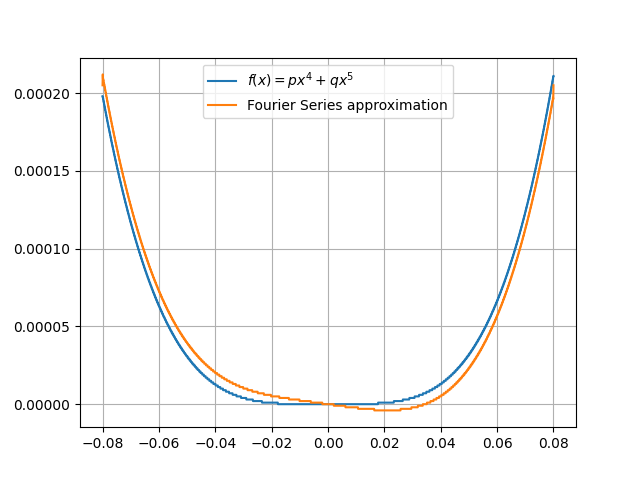
\includegraphics[width=\linewidth]{2023/CE/25/figs/Figure_1.png}
    \caption{Fourier Series Approximation of $f\brak{x}$ for $p=5$, $q=2$, $L=0.08$}
\end{figure}

\newpage
\item A continuous real-valued signal $x\brak{t}$ has finite positive energy and $x\brak{t} = 0$, $\forall$ $t < 0$. From the list given below, select ALL the signals whose
continuous-time Fourier transform is purely imaginary.\\
\begin{enumerate}
\item$x\brak{t} + x\brak{-t}$
\item$x\brak{t} - x\brak{-t}$
\item$j\brak{x\brak{t} + x\brak{-t}}$
\item$j\brak{x\brak{t} - x\brak{-t}}$
\end{enumerate}
\hfill{(GATE IN 2023)}\\
\solution
\iffalse
\let\negmedspace\undefined
\let\negthickspace\undefined
\documentclass[journal,12pt,twocolumn]{IEEEtran}
\usepackage{cite}
\usepackage{amsmath,amssymb,amsfonts,amsthm}
\usepackage{algorithmic}
\usepackage{graphicx}
\usepackage{textcomp}
\usepackage{xcolor}
\usepackage{txfonts}
\usepackage{listings}
\usepackage{enumitem}
\usepackage{mathtools}
\usepackage{gensymb}
\usepackage{comment}
\usepackage[breaklinks=true]{hyperref}
\usepackage{tkz-euclide} 
\usepackage{listings}
\usepackage{gvv}                                        
\def\inputGnumericTable{}                                 
\usepackage[latin1]{inputenc}                                
\usepackage{color}                                            
\usepackage{array}                                            
\usepackage{longtable}                                       
\usepackage{calc}                                             
\usepackage{multirow}                                         
\usepackage{hhline}                                           
\usepackage{ifthen}                                           
\usepackage{lscape}

\newtheorem{theorem}{Theorem}[section]
\newtheorem{problem}{Problem}
\newtheorem{proposition}{Proposition}[section]
\newtheorem{lemma}{Lemma}[section]
\newtheorem{corollary}[theorem]{Corollary}
\newtheorem{example}{Example}[section]
\newtheorem{definition}[problem]{Definition}
\newcommand{\BEQA}{\begin{eqnarray}}
\newcommand{\EEQA}{\end{eqnarray}}
\newcommand{\define}{\stackrel{\triangle}{=}}
\theoremstyle{remark}
\newtheorem{rem}{Remark}
\begin{document}
\bibliographystyle{IEEEtran}
\vspace{3cm}
\title{\textbf{IN-2023}}
\author{EE23BTECH11210-Dhyana Teja Machineni$^{*}$% <-this % stops a space
}
\maketitle
\newpage
\bigskip

\textbf{QUESTION:}\\
A continuous real-valued signal $x\brak{t}$ has finite positive energy and $x\brak{t} = 0$, $\forall$ $t < 0$. From the list given below, select ALL the signals whose
continuous-time Fourier transform is purely imaginary.\\
\begin{enumerate}
\item$x\brak{t} + x\brak{-t}$
\item$x\brak{t} - x\brak{-t}$
\item$j\brak{x\brak{t} + x\brak{-t}}$
\item$j\brak{x\brak{t} - x\brak{-t}}$
\end{enumerate}
\hfill{(GATE IN 2023)}\\
\solution\\
\fi
\begin{table}[h]
         \renewcommand{\arraystretch}{1.5}
\begin{tabular}{|c|c|}
\hline
Parameter & Description  \\\hline
$x(t)$ & Continuous real valued signal  \\\hline
$t$ & time \\\hline
$f$ & frequency of the signal \\\hline
$Y(f)$& Fourier Transfom of $y(t)$\\\hline
\end{tabular}

         \caption{Variables and their descriptions}
     \end{table}\\
Fourier transform of a signal $y\brak{t}$\\
\begin{align}
\mathcal{F}\{y(t)\} &= Y\brak{f}\\
Y\brak{f}&=\int_{-\infty}^{\infty} y\brak{t} e^{-j 2\pi f t} \ dt\\
Y^*\brak{f}&=\int_{-\infty}^{\infty} y^*\brak{t} e^{j 2\pi f t} \ dt
\end{align}
Fourier transform is purely imaginary if $Y\brak{f}+Y^*\brak{f}=0$\\
\begin{enumerate}
\item $x\brak{t} + x\brak{-t}$\\
\begin{align}
 y\brak{t}&=x\brak{t} + x\brak{-t}\\
 y^*\brak{t}&=y\brak{t}\\
 y\brak{t}&=y\brak{-t}\\
 Y\brak{f}+Y^*\brak{f}&=\int_{-\infty}^{\infty} y\brak{t} e^{-j 2\pi f t} \ dt+\int_{-\infty}^{\infty} y^*\brak{t} e^{j 2\pi f t} \ dt\\
 &=2\int_{-\infty}^{\infty} y\brak{t} cos\brak{2 \pi ft} \ dt
\end{align}
$\therefore$ Fourier Transform is Purely real.\\
\item $x\brak{t} - x\brak{-t}$\\
\begin{align}
  y\brak{t}&=x\brak{t} - x\brak{-t}\\
  y^*\brak{t}&=y\brak{t}=-y\brak{-t}\\
  Y\brak{f}&=\int_{-\infty}^{\infty} y\brak{t} e^{-j 2\pi f t} \ dt\\
  Y^*\brak{f}&=-\int_{-\infty}^{\infty} y\brak{-t} e^{j 2\pi f t} \ dt\\
  &=-\int_{-\infty}^{\infty} y\brak{t} e^{-j 2\pi f t} \ dt\\
  Y\brak{f}+Y^*\brak{f}&=0
\end{align}
$\therefore$ Fourier Transform is purely imaginary.\\
\item $j\brak{x\brak{t} + x\brak{-t}}$
\begin{align}
  y\brak{t}&= j\brak{x\brak{t} + x\brak{-t}}\\
  y\brak{-t}&=y\brak{t}\\
  y^*\brak{t}&=-y(t)\\
  Y\brak{f}&=\int_{-\infty}^{\infty} y\brak{t} e^{-j 2\pi f t} \ dt\\
  Y^*\brak{f}&=-\int_{-\infty}^{\infty} y\brak{t} e^{j 2\pi f t} \ dt\\
  &=-\int_{-\infty}^{\infty} y\brak{t} e^{-j 2\pi f t} \ dt\\
  Y\brak{f}+Y^*\brak{f}&=0
\end{align}
$\therefore$ Fourier Transform is Purely imaginary.\\
\item $j\brak{x\brak{t} - x\brak{-t}}$
\begin{align}
  y\brak{t}&=j\brak{x\brak{t} - x\brak{-t}}\\
  y\brak{-t}&=-y\brak{t}\\
  y^*\brak{t}&=-y\brak{t}\\
  Y\brak{f}&=\int_{-\infty}^{\infty} y\brak{t} e^{-j 2\pi f t} \ dt\\
  Y^*\brak{f}&=-\int_{-\infty}^{\infty} y\brak{t} e^{j 2\pi f t} \ dt\\
  &=\int_{-\infty}^{\infty} y\brak{t} e^{-j 2\pi f t} \ dt\\
  Y\brak{f}+Y^*\brak{f}&=2\int_{-\infty}^{\infty} y\brak{t} e^{-j 2\pi f t} \ dt
  \end{align}
$\therefore$ Fourier Transform is not Purely imaginary.\\
\end{enumerate}
%\end{document}

\item Let $x_1(t) = u(t + 1.5) - u(t - 1.5)$ and $x_2(t)$ is shown in the figure below. For $y(t) = x_1(t) * x_2(t)$, the $\int_{-\infty}^{\infty} y(t) \, dt$ is \underline{\hspace{2cm}}.\\

\begin{figure}[htbp]
    \centering
    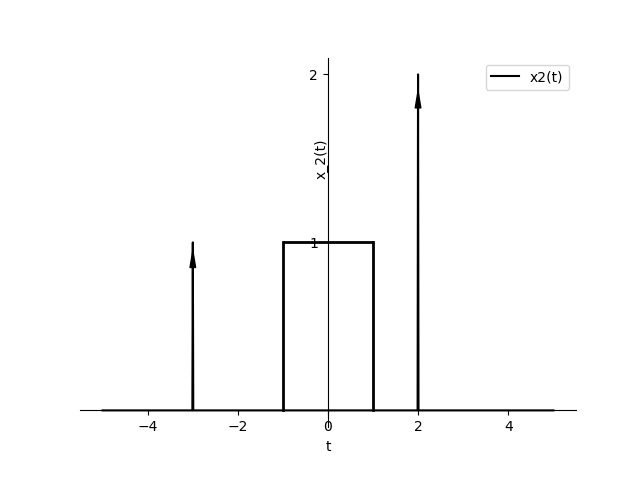
\includegraphics[width=0.5\textwidth]{2023/EC/58/figs/gatefig.png}
    \caption{Figure}
    \label{fig:graph}
\end{figure}

\hfill{(GATE IN 2023)}\\
\solution
\iffalse
\let\negmedspace\undefined
\let\negthickspace\undefined
\documentclass[journal,12pt,onecolumn]{IEEEtran}
\usepackage{cite}
\usepackage{amsmath,amssymb,amsfonts,amsthm}
\usepackage{algorithmic}
\usepackage{graphicx}
\usepackage{textcomp}
\usepackage{xcolor}
\usepackage{txfonts}
\usepackage{listings}
\usepackage{enumitem}
\usepackage{mathtools}
\usepackage{gensymb}

\usepackage{tkz-euclide} % loads  TikZ and tkz-base
\usepackage{listings}



\newtheorem{theorem}{Theorem}[section]
\newtheorem{problem}{Problem}
\newtheorem{proposition}{Proposition}[section]
\newtheorem{lemma}{Lemma}[section]
\newtheorem{corollary}[theorem]{Corollary}
\newtheorem{example}{Example}[section]
\newtheorem{definition}[problem]{Definition}
%\newtheorem{thm}{Theorem}[section] 
%\newtheorem{defn}[thm]{Definition}
%\newtheorem{algorithm}{Algorithm}[section]
%\newtheorem{cor}{Corollary}
\newcommand{\BEQA}{\begin{eqnarray}}
\newcommand{\EEQA}{\end{eqnarray}}
\newcommand{\system}[1]{\stackrel{#1}{\rightarrow}}

\newcommand{\define}{\stackrel{\triangle}{=}}
\theoremstyle{remark}
\newtheorem{rem}{Remark}
%\bibliographystyle{ieeetr}
\begin{document}
%
\providecommand{\pr}[1]{\ensuremath{\Pr\left(#1\right)}}
\providecommand{\prt}[2]{\ensuremath{p_{#1}^{\left(#2\right)} }}        % own macro for this question
\providecommand{\qfunc}[1]{\ensuremath{Q\left(#1\right)}}
\providecommand{\sbrak}[1]{\ensuremath{{}\left[#1\right]}}
\providecommand{\lsbrak}[1]{\ensuremath{{}\left[#1\right.}}
\providecommand{\rsbrak}[1]{\ensuremath{{}\left.#1\right]}}
\providecommand{\brak}[1]{\ensuremath{\left(#1\right)}}
\providecommand{\lbrak}[1]{\ensuremath{\left(#1\right.}}
\providecommand{\rbrak}[1]{\ensuremath{\left.#1\right)}}
\providecommand{\cbrak}[1]{\ensuremath{\left\{#1\right\}}}
\providecommand{\lcbrak}[1]{\ensuremath{\left\{#1\right.}}
\providecommand{\rcbrak}[1]{\ensuremath{\left.#1\right\}}}
\newcommand{\sgn}{\mathop{\mathrm{sgn}}}
\providecommand{\abs}[1]{\left\vert#1\right\vert}
\providecommand{\res}[1]{\Res\displaylimits_{#1}} 
\providecommand{\norm}[1]{\left\lVert#1\right\rVert}
%\providecommand{\norm}[1]{\lVert#1\rVert}
\providecommand{\mtx}[1]{\mathbf{#1}}
\providecommand{\mean}[1]{E\left[ #1 \right]}
\providecommand{\cond}[2]{#1\middle|#2}
\providecommand{\fourier}{\overset{\mathcal{F}}{ \rightleftharpoons}}
\newenvironment{amatrix}[1]{%
  \left(\begin{array}{@{}*{#1}{c}|c@{}}
}{%
  \end{array}\right)
}
%\providecommand{\hilbert}{\overset{\mathcal{H}}{ \rightleftharpoons}}
%\providecommand{\system}{\overset{\mathcal{H}}{ \longleftrightarrow}}
    %\newcommand{\solution}[2]{\textbf{Solution:}{#1}}
\newcommand{\solution}{\noindent \textbf{Solution: }}
\newcommand{\cosec}{\,\text{cosec}\,}
\providecommand{\dec}[2]{\ensuremath{\overset{#1}{\underset{#2}{\gtrless}}}}
\newcommand{\myvec}[1]{\ensuremath{\begin{pmatrix}#1\end{pmatrix}}}
\newcommand{\mydet}[1]{\ensuremath{\begin{vmatrix}#1\end{vmatrix}}}
\newcommand{\myaugvec}[2]{\ensuremath{\begin{amatrix}{#1}#2\end{amatrix}}}
\providecommand{\rank}{\text{rank}}
\providecommand{\pr}[1]{\ensuremath{\Pr\left(#1\right)}}
\providecommand{\qfunc}[1]{\ensuremath{Q\left(#1\right)}}
    \newcommand*{\permcomb}[4][0mu]{{{}^{#3}\mkern#1#2_{#4}}}
\newcommand*{\perm}[1][-3mu]{\permcomb[#1]{P}}
\newcommand*{\comb}[1][-1mu]{\permcomb[#1]{C}}
\providecommand{\qfunc}[1]{\ensuremath{Q\left(#1\right)}}
\providecommand{\gauss}[2]{\mathcal{N}\ensuremath{\left(#1,#2\right)}}
\providecommand{\diff}[2]{\ensuremath{\frac{d{#1}}{d{#2}}}}
\providecommand{\myceil}[1]{\left \lceil #1 \right \rceil }
\newcommand\figref{Fig.~\ref}
\newcommand\tabref{Table~\ref}
\newcommand{\sinc}{\,\text{sinc}\,}
\newcommand{\rect}{\,\text{rect}\,}
%%
%   %\newcommand{\solution}[2]{\textbf{Solution:}{#1}}
%\newcommand{\solution}{\noindent \textbf{Solution: }}
%\newcommand{\cosec}{\,\text{cosec}\,}
%\numberwithin{equation}{section}
%\numberwithin{equation}{subsection}
%\numberwithin{problem}{section}
%\numberwithin{definition}{section}
%\makeatletter
%\@addtoreset{figure}{problem}
%\makeatother

%\let\StandardTheFigure\thefigure
\let\vec\mathbf


\bibliographystyle{IEEEtran}
\title{Gate 2023 EC 58}
\author{HIBA MUHAMMED\\
        EE23BTECH11026}
\maketitle

\section*{Problem Statement}
Let $x_1(t) = u(t + 1.5) - u(t - 1.5)$ and $x_2(t)$ is shown in the figure below. For $y(t) = x_1(t) * x_2(t)$, the $\int_{-\infty}^{\infty} y(t) \, dt$ is \underline{\hspace{2cm}}.

\begin{figure}[htbp]
    \centering
    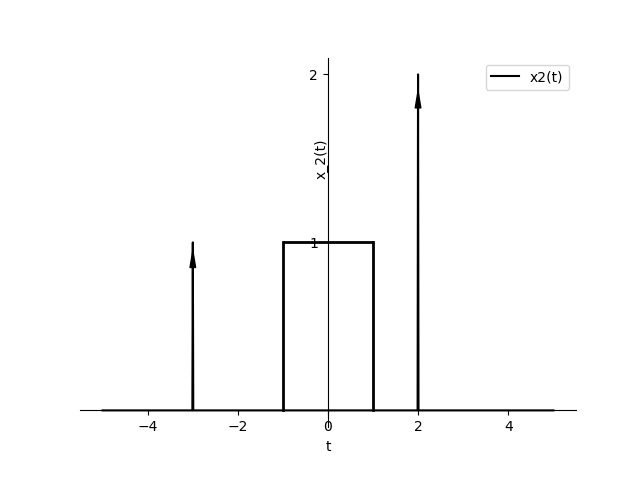
\includegraphics[width=0.5\textwidth]{2023/EC/58/figs/gatefig.png}
    \caption{Figure}
    \label{fig:graph}
\end{figure}

\section*{Solution}
\fi
\begin{table}[htbp]
    \centering
        \begin{tabular}{|c|c|p{6cm}|}
        \hline
        \multicolumn{3}{|c|}{\textbf{Input Parameters}} \\
        \hline
        \textbf{Function} & \textbf{Expression} & \textbf{Description} \\
        \hline
        $x_1(t)$ & $u(t + 1.5) - u(t - 1.5)$ & Step function with delay and width parameters. \\
        \hline
        $X_1(f)$ &  & Fourier Transform of $x_1(t)$. \\
        \hline
        $x_2(t)$ & $\delta(t + 3) + \text{rect}\left(\frac{t}{2}\right) + 2\delta(t - 2)$ & Impulse function followed by a rectangle and two impulses. \\
        \hline
        $X_2(f)$ &  & Fourier Transform of $x_2(t)$. \\
        \hline
    \end{tabular}


    \caption{Input Parameters}
    \label{tab:gate_58table}
\end{table}

\begin{align}
x_1(t) &= u(t+1.5) - u(t-1.5) \\
x_1(t) &= \text{rect}\left(\frac{t}{3}\right) \\
\end{align}


The Fourier Transform of $rect\left(\frac{t}{a}\right)$:

\begin{align}
\text{rect}\left(\frac{t}{a}\right) &\xleftrightarrow{\mathcal{F}} a \times \sin(2\pi f \frac{a}{2}) \\
\text{where } \text{rect}\left(\frac{t}{a}\right) &= \begin{cases}
1 & \text{if } |t| < \frac{a}{2} \\
0 & \text{otherwise}
\end{cases}\\
& X_1(f)=3\text{sinc}(1.5\cdot 2\pi f) & \\
& x_2(t) = \delta(t+3) + \text{rect}\left(\frac{t}{2}\right) + 2\delta(t-2) & \\
& X_2(f) = e^{3j\cdot 2\pi f} + 2\text{sinc}(2\pi f) + 2e^{-2j \cdot 2\pi f} & \\
& Y(f) = X_1(f) \cdot X_2(f) \\
& Y(f)= 3\text{sinc}(1.5 \cdot 2\pi f) \cdot (e^{3j \cdot 2\pi f} + 2\text{sinc}(2\pi f) + 2e^{-2j \cdot 2\pi f})\\
& y(t) = x_1(t) * x_2(t) \\
& Y(f) \xleftrightarrow{\mathcal{F}} y(t)\\
& y(t) = \text{rect}\left(\frac{t+3}{3}\right) + 2\text{rect}\left(\frac{t-2}{3}\right) + (t+2.5)u(t+2.5) + (t-2.5)u(t-2.5) \\
& - (t+0.5)u(t+0.5) - (t-0.5)u(t-0.5)\\
& Y(f) = \int_{-\infty}^{\infty} y(t) e^{-j2\pi ft} \, dt\\
& \int_{-\infty}^{\infty} y(t) \, dt = Y(0)\\
& Y(0)= 3\text{sinc}(0) \cdot (e^{0} + 2\text{sinc}(0) + 2e^{0}) \\
&\hspace{1cm}= 3\cdot (1 + 2 + 2) \\
&\hspace{1cm}= 15
\end{align}



Therefore, the value of $\int_{-\infty}^{\infty} y(t) \, dt$ is $15$


\begin{figure}[htbp]
    \centering
    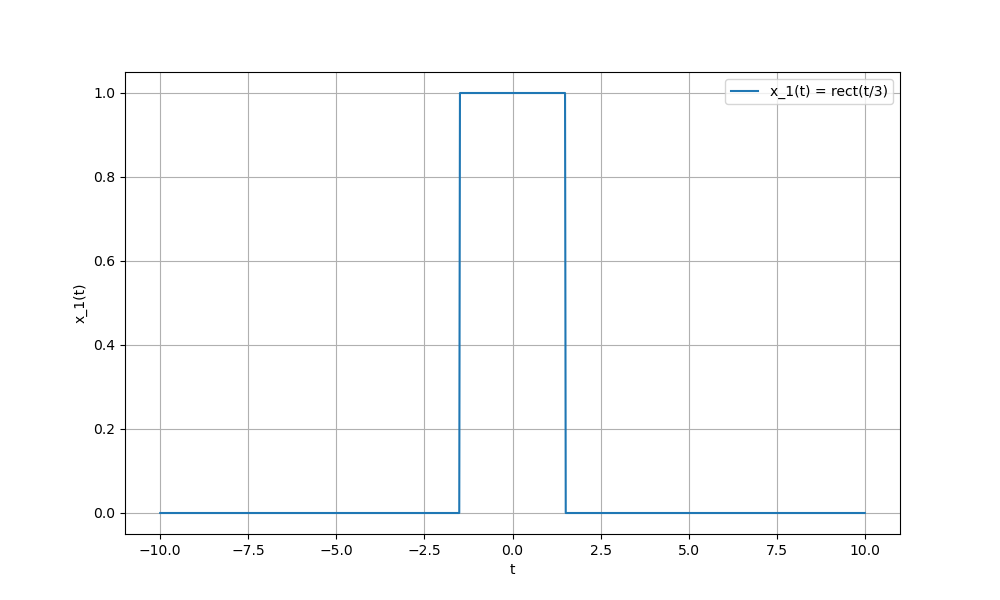
\includegraphics[width=0.8\textwidth]{2023/EC/58/figs/gate_x1.png}
    \caption{Graph of \(x_1(t) = \text{rect}\left(\frac{t}{3}\right)\)}
    \label{fig:x_1_graph}
\end{figure}


\begin{figure}[htbp]
    \centering
    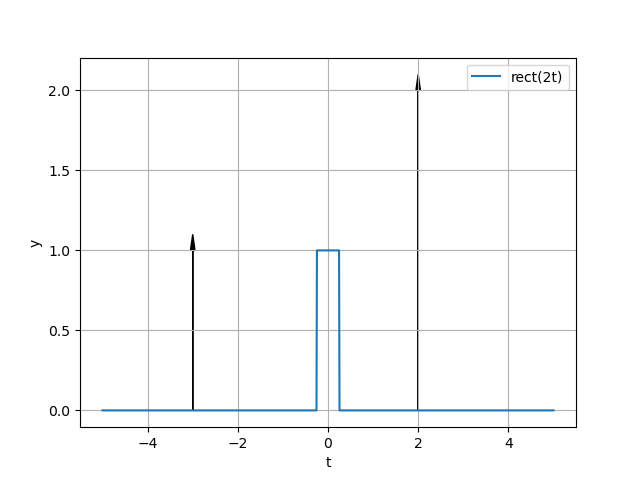
\includegraphics[width=0.8\textwidth]{2023/EC/58/figs/gate_x2.png}
    \caption{Graph of \(x_2(t) = \delta(t+3) + \text{rect}(2t) + 2\delta(t-2)\)}
    \label{fig:x_2_graph}
\end{figure}


\begin{figure}[htbp]
    \centering
    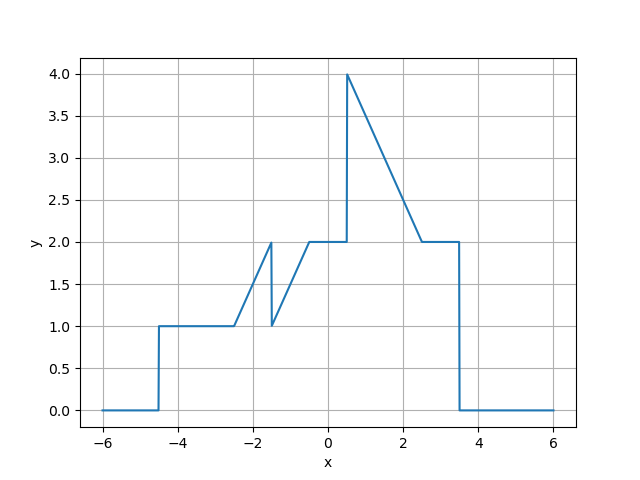
\includegraphics[width=0.8\textwidth]{2023/EC/58/figs/gate_y.png}
    \caption{Graph of \(y(t)\)}
    \label{fig:x_2_graph}
\end{figure}
%\end{document}

\pagebreak
\item Consider a discrete-time signal with period $N=5$. Let the discrete-time Fourier series (DTFS) representation be $ x[n] = \sum\limits_{k=0}^{4} a_k e^{\frac{jk2\pi n}{5}} $where $a_0=1$, $a_1=3j$, $a_2=2j$, $a_3=-2j$, $a_4=-3j$. The value of the sum $\sum\limits_{n=0}^{4}x[n] \sin\left(\frac{4\pi n}{5}\right) $is\\
(A) -10\\
(B) 10\\
(C) -2\\
(D) 2\\
\hfill Gate 2023 EC 47
\solution
\pagebreak

\item A continuous time, band-limited signal $x(t)$ has its Fourier transform described by:
\[ X(f) = \begin{cases} 
1 - \frac{|f|}{200} & \text{if } |f| \leq 200 \\
0 & \text{if } |f| > 200 
\end{cases} \]
The signal is uniformly sampled at a sampling rate of 600 Hz. The Fourier transform of the signal is $X_s(f)$. What is the value of $\frac{X_s(600)}{X_s(500)}$? \\\hfill{(GATE 2023 BM)}
\solution
\let\negmedspace\undefined
\let\negthickspace\undefined
\documentclass[journal,12pt,twocolumn]{IEEEtran}

\usepackage{cite}
\usepackage{amsmath,amssymb,amsfonts,amsthm}
\usepackage{graphicx}
\usepackage{textcomp}
\usepackage{xcolor}
\usepackage{txfonts}
\usepackage{listings}
\usepackage{enumitem}
\usepackage{mathtools}
\usepackage{gensymb}
\usepackage[breaklinks=true]{hyperref}
\usepackage{tkz-euclide} % loads  TikZ and tkz-base
\usepackage{listings}
\usepackage{circuitikz}
\usepackage{graphicx}

%\newcounter{MYtempeqncnt}
\DeclareMathOperator*{\Res}{Res}
%\renewcommand{\baselinestretch}{2}
\renewcommand\thesection{\arabic{section}}
\renewcommand\thesubsection{\thesection.\arabic{subsection}}
\renewcommand\thesubsubsection{\thesubsection.\arabic{subsubsection}}

\renewcommand\thesectiondis{\arabic{section}}
\renewcommand\thesubsectiondis{\thesectiondis.\arabic{subsection}}
\renewcommand\thesubsubsectiondis{\thesubsectiondis.\arabic{subsubsection}}

% correct bad hyphenation here
\hyphenation{op-tical net-works semi-conduc-tor}
\def\inputGnumericTable{}                                 %%

\lstset{
	frame=single,
	breaklines=true,
	columns=fullflexible
}



\newtheorem{theorem}{Theorem}[section]
\newtheorem{problem}{Problem}
\newtheorem{proposition}{Proposition}[section]
\newtheorem{lemma}{Lemma}[section]
\newtheorem{corollary}[theorem]{Corollary}
\newtheorem{example}{Example}[section]
\newtheorem{definition}[problem]{Definition}
\newcommand{\BEQA}{\begin{eqnarray}}
	\newcommand{\EEQA}{\end{eqnarray}}
\newcommand{\define}{\stackrel{\triangle}{=}}
\newcommand\figref{Fig.~\ref}
\newcommand\tabref{Table~\ref}
\bibliographystyle{IEEEtran}
%\bibliographystyle{ieeetr}


\providecommand{\mbf}{\mathbf}
\providecommand{\pr}[1]{\ensuremath{\Pr\left(#1\right)}}
\providecommand{\qfunc}[1]{\ensuremath{Q\left(#1\right)}}
\providecommand{\sbrak}[1]{\ensuremath{{}\left[#1\right]}}
\providecommand{\lsbrak}[1]{\ensuremath{{}\left[#1\right.}}
\providecommand{\rsbrak}[1]{\ensuremath{{}\left.#1\right]}}
\providecommand{\brak}[1]{\ensuremath{\left(#1\right)}}
\providecommand{\lbrak}[1]{\ensuremath{\left(#1\right.}}
\providecommand{\rbrak}[1]{\ensuremath{\left.#1\right)}}
\providecommand{\cbrak}[1]{\ensuremath{\left\{#1\right\}}}
\providecommand{\lcbrak}[1]{\ensuremath{\left\{#1\right.}}
\providecommand{\rcbrak}[1]{\ensuremath{\left.#1\right\}}}
\theoremstyle{remark}
\newtheorem{rem}{Remark}
\newcommand{\sgn}{\mathop{\mathrm{sgn}}}
\providecommand{\abs}[1]{\left\vert#1\right\vert}
\providecommand{\res}[1]{\Res\displaylimits_{#1}}
\providecommand{\norm}[1]{\left\lVert#1\right\rVert}
%\providecommand{\norm}[1]{\lVert#1\rVert}
\providecommand{\mtx}[1]{\mathbf{#1}}
\providecommand{\mean}[1]{E\left[ #1 \right]}
\providecommand{\fourier}{\overset{\mathcal{F}}{ \rightleftharpoons}}
%\providecommand{\hilbert}{\overset{\mathcal{H}}{ \rightleftharpoons}}
\providecommand{\system}{\overset{\mathcal{H}}{ \longleftrightarrow}}
%\newcommand{\solution}[2]{\textbf{Solution:}{#1}}
\newcommand{\solution}{\noindent \textbf{Solution: }}
\newcommand{\cosec}{\,\text{cosec}\,}
\providecommand{\dec}[2]{\ensuremath{\overset{#1}{\underset{#2}{\gtrless}}}}
\newcommand{\myvec}[1]{\ensuremath{\begin{pmatrix}#1\end{pmatrix}}}
\newcommand{\mydet}[1]{\ensuremath{\begin{vmatrix}#1\end{vmatrix}}}
\renewcommand{\abstractname}{Question}

\let\vec\mathbf

	
	\vspace{3cm}
	
	


\newcommand{\permcomb}[4][0mu]{{{}^{#3}\mkern#1#2_{#4}}}
\newcommand{\comb}[1][-1mu]{\permcomb[#1]{C}}

%\IEEEpeerreviewmaketitle

\newcommand \tab [1][1cm]{\hspace*{#1}}
%\newcommand{\Var}{$\sigma ^2$}
\usepackage{amssymb}
\usepackage{amsmath}
\title{
	
\title{GATE 2023 BM 33}
\author{EE23BTECH11213 - MUTHYALA NIKHITHA SRI
}


}
\begin{document}

\maketitle

\textbf{Question:} 
A continuous time, band-limited signal $x\brak{t}$ has its Fourier transform described by:\\
\begin{equation}
 X\brak{f} = \begin{cases} 
1 - \frac{\abs{f}}{200} & \text{if } \abs{f} \leq 200 \\
0 & \text{if } \abs{f} > 200 \label{eq: 1404}
\end{cases}  \\
\end{equation}
The signal is uniformly sampled at a sampling rate of 600 Hz. The Fourier transform of the signal is $X_s\brak{f}$. What is the value of $\frac{X_s\brak{600}}{X_s\brak{500}}$? \\

\textbf{Solution: }

\begin{table}[h]
 	\centering
 	\resizebox{6 cm}{!}{
 		\begin{tabular}{|c|c|c|} 
    \hline
    \textbf{Variable} & \textbf{Description} & \textbf{Value} \\
    \hline
    $x(t)$ & input function & none \\
    \hline
    $y(t)$ & output function & $\sin(\pi t)$ \\
    \hline
    $H(s)$ & Transfer-function & $\frac{s-\pi}{s+\pi}$ \\
    \hline
\end{tabular}

 	}
 	\caption{Input Parameters}
    \label{tab:table_33}
 \end{table}

\begin{align} 
X_s\brak{f} &= \frac{1}{600} \sum_{k=-\infty}^{\infty} X\brak{f - 600k} \\
\implies X_s\brak{f+600} &= \frac{X\brak{f}}{600} \end{align} Using \eqref{eq: 1404}
\begin{align} 
X_s\brak{600} &= \frac{X\brak{0}}{600} \\
\implies X_s\brak{600} &= \frac{1}{600} \\
X_s\brak{500} &= \frac{X\brak{-100}}{600} \\
\implies X_s\brak{500} &= \frac{1}{2\cdot 600} \\
\frac{X_s\brak{600}}{X_s\brak{500}} &= 2 
\end{align}

\begin{figure}[h!]
    \centering
    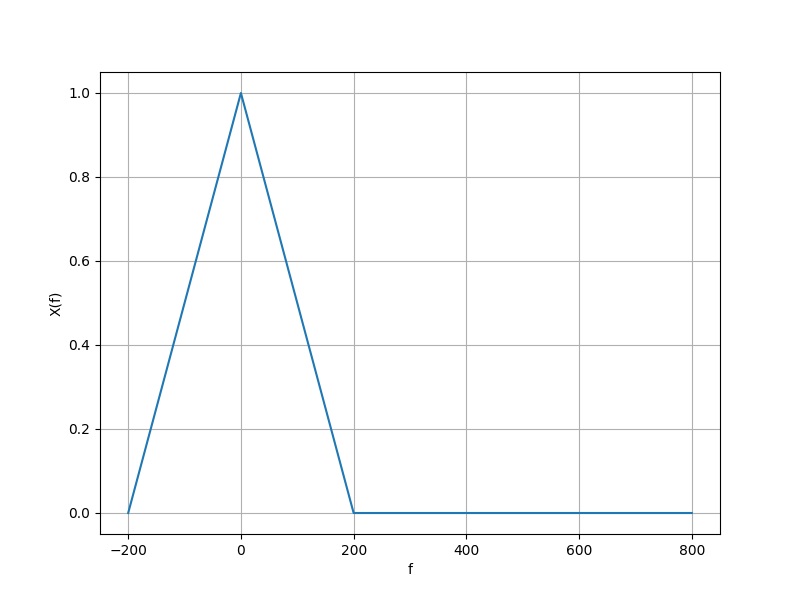
\includegraphics[width=\columnwidth]{figs/f1.png}
    \caption{Plot of $X\brak{f}$}
    \label{fig:nikh1}
\end{figure}

\begin{figure}[h!]
    \centering
    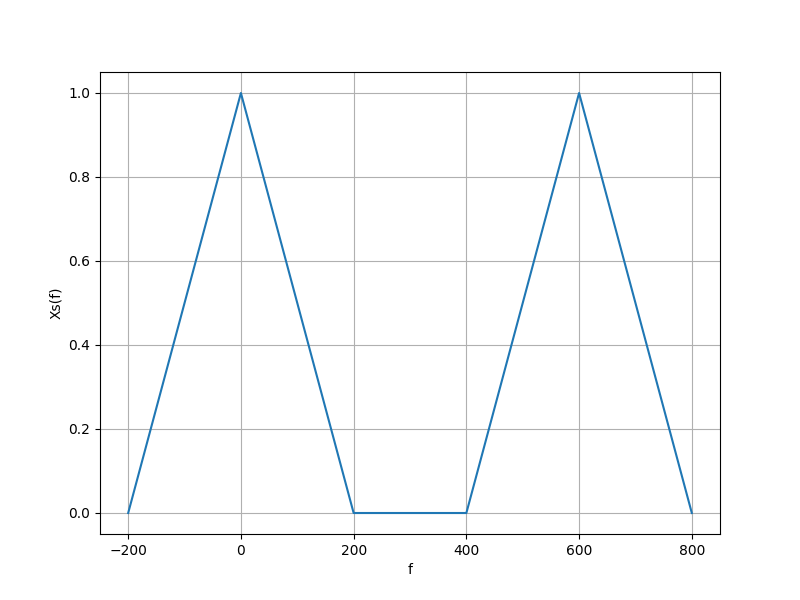
\includegraphics[width=\columnwidth]{figs/f2.png}
    \caption{Plot of $X_s\brak{f}$}
    \label{fig:nikh2}
\end{figure}


\end{document}

\pagebreak

 \item The magnitude and phase plots of an LTI systems are shown in figure. Find the transfer function.
\begin{figure}[!h]
    \centering
    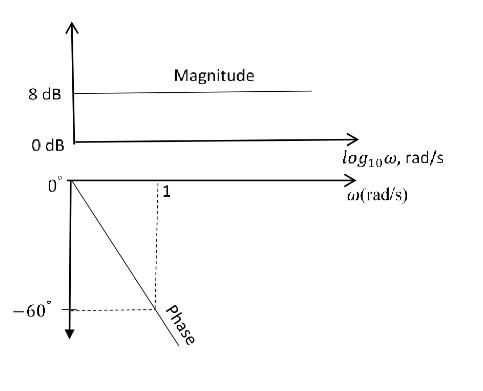
\includegraphics[width=\columnwidth]{2023/EE/36/figs/gate.png}
    \caption{}
    \label{fig:EEgatefig36.23}
\end{figure}
\begin{enumerate}
    \item $2.511 e^{-0.0032s}$\\
    \item $\frac{e^{-2.514s}}{s+1}$\\
    \item $1.04e^{-2.514s}$\\
    \item $2.511 e^{-1.047s}$\\
\end{enumerate} \hfill{(GATE EE 23)}\\

\solution
\iffalse
\documentclass[journal,12pt,twocolumn]{IEEEtran}
\usepackage{cite}
\usepackage{amsmath,amssymb,amsfonts,amsthm}
\usepackage{algorithmic}
\usepackage{graphicx}
\usepackage{textcomp}
\usepackage{xcolor}
\usepackage{txfonts}
\usepackage{listings}
\usepackage{enumitem}
\usepackage{mathtools}
\usepackage{gensymb}
\usepackage{comment}
\usepackage[breaklinks=true]{hyperref}
\usepackage{tkz-euclide}
\usepackage{listings}
\usepackage{gvv}
\def\inputGnumericTable{}
\usepackage[latin1]{inputenc}
\usepackage{color}
\usepackage{array}
\usepackage{longtable}
\usepackage{calc}
\usepackage{multirow}
\usepackage{hhline}
\usepackage{ifthen}
\usepackage{lscape}

\newtheorem{theorem}{Theorem}[section]
\newtheorem{problem}{Problem}
\newtheorem{proposition}{Proposition}[section]
\newtheorem{lemma}{Lemma}[section]
\newtheorem{corollary}[theorem]{Corollary}
\newtheorem{example}{Example}[section]
\newtheorem{definition}[problem]{Definition}
\newcommand{\BEQA}{\begin{eqnarray}}
    \newcommand{\EEQA}{\end{eqnarray}}
\newcommand{\define}{\stackrel{\triangle}{=}}
\theoremstyle{remark}
\newtheorem{rem}{Remark}
\begin{document}
    
    \bibliographystyle{IEEEtran}
    \vspace{3cm}
    
    \title{Gate 2023 EE Q36}
    \author{EE23BTECH11212 - Manugunta Meghana Sai$^{*}$% <-this % stops a space
    }
    \maketitle
    \newpage
    \bigskip
    
    \renewcommand{\thefigure}{\theenumi}
    \renewcommand{\thetable}{\theenumi}
    
    \vspace{3cm}
    \textbf{Gate 2023 EE Q36} 
    The magnitude and phase plots of an LTI systems are shown in figure. Find the transfer function.\\
    \begin{figure}[h!]
        \centering
        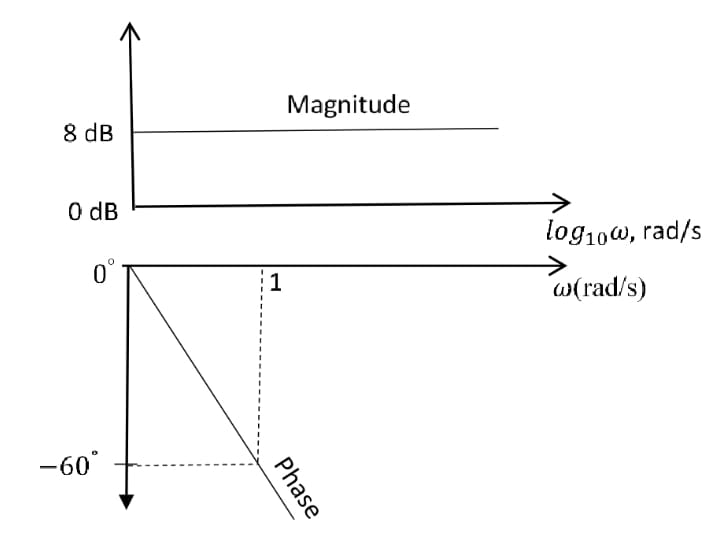
\includegraphics[width=\columnwidth]{figs/gate.jpeg}
        \caption{Graphs}
        \label{fig:1ee36}
    \end{figure}
    \begin{enumerate}
        \item $2.511 e^{-0.0032s}$\\
        \item $\frac{e^{-2.514s}}{s+1}$\\
        \item $1.04e^{-2.514s}$\\
        \item $2.511 e^{-1.047s}$\\
    \end{enumerate}
    
    \solution
    \fi
    From~\figref{fig:EEgatefig36.23}
    \begin{align}
        \abs{{H}\brak{j\omega}}&= 8 \\
        \angle H\brak{j\omega} &= \frac{-\pi}{3} \omega
    \end{align}
    Substituting the values from~\figref{fig:EEgatefig36.23}, magnitude of transfer function is:
    \begin{align}
        8 &= 20\log_{10}(\abs{{H}\brak{j\omega}})\\
        \abs{{H}\brak{j\omega}} &= 10^{0.4} = 2.511
    \end{align}
    Substituting the values from~\figref{fig:EEgatefig36.23}, The direction of the transfer function is:
    \begin{align}
        \frac{H\brak{j\omega}}{\abs{{H}\brak{j\omega}}} = e^{-j\frac{\pi}{3}\omega}
    \end{align}
    \begin{align}
        H\brak{j\omega} &= 2.511 e^{-j\frac{\pi}{3}\omega} \\
        &= 2.511 e^{-1.047s}
    \end{align}
    \setcounter{figure}{1} 
%\end{document}


\newpage
\item The value of the convolution of $f(x) = 3\cos(2x)$ and $g(x) = \frac{1}{3}\sin(2x)$ where $x \in [0, 2\pi)$, at $x = \frac{\pi}{3}$, is (Rounded off to 2 decimal places)\\
\hfill (GATE 2023 GE)\\
\solution
\pagebreak
\item A system is described by the following differential equation
    \[
    0.01 \frac{d^2y(t)}{dt^2} + 0.2\frac{dy(t)}{dt} + y(t) = 6x(t)
    \]
    where time \( t \) is in seconds. If \( x(t) \) is the unit step input applied at \( t = 0 \) s to this system, the magnitude of the output at \( t = 1 \) s is \(\underline{\hspace{2cm}}\). (Round off the answer to two decimal places.)
    \hfill (GATE-2023.BM)\\
    \solution
    \pagebreak

\item In the differential equation $\frac{dy}{dx} + \alpha x y = 0, \alpha$ is a positive constant. If $y = 1.0$ at
$x = 0.0$, and $y = 0.8$ at $x = 1.0$, the value of $\alpha$ is (rounded off to three decimal places).  \hfill(GATE CE 30 2023)\\
\solution
\iffalse
\documentclass[journal,12pt,twocolumn]{IEEEtran}
\usepackage{cite}
\usepackage{amsmath,amssymb,amsfonts,amsthm}
\usepackage{algorithmic}
\usepackage{graphicx}
\usepackage{textcomp}
\usepackage{xcolor}
\usepackage{txfonts}
\usepackage{listings}
\usepackage{enumitem}
\usepackage{mathtools}
\usepackage{gensymb}
\usepackage{comment}
\usepackage[breaklinks=true]{hyperref}
\usepackage{tkz-euclide}
\usepackage{listings}
\usepackage{gvv}
\def\inputGnumericTable{}
\usepackage[latin1]{inputenc}
\usepackage{color}
\usepackage{array}
\usepackage{longtable}
\usepackage{calc}
\usepackage{multirow}
\usepackage{hhline}
\usepackage{ifthen}
\usepackage{lscape}
\usepackage{caption}

\newtheorem{theorem}{Theorem}[section]
\newtheorem{problem}{Problem}
\newtheorem{proposition}{Proposition}[section]
\newtheorem{lemma}{Lemma}[section]
\newtheorem{corollary}[theorem]{Corollary}
\newtheorem{example}{Example}[section]
\newtheorem{definition}[problem]{Definition}
\newcommand{\BEQA}{\begin{eqnarray}}
\newcommand{\EEQA}{\end{eqnarray}}
\newcommand{\define}{\stackrel{\triangle}{=}}
\theoremstyle{remark}
\newtheorem{rem}{Remark}
\begin{document}

\bibliographystyle{IEEEtran}
\vspace{3cm}

\title{GATE: CE - 30.2023}
\author{EE23BTECH11010 - Venkatesh D Bandawar $^{*}$% <-this % stops a space
}
\maketitle
% \newpage
\bigskip

% \renewcommand{\thefigure}{\theenumi}
% \renewcommand{\thetable}{\theenumi}

\textbf{Question:} In the differential equation $\frac{dy}{dx} + \alpha x y = 0, \alpha$ is a positive constant. If $y = 1.0$ at
$x = 0.0$, and $y = 0.8$ at $x = 1.0$, the value of $\alpha$ is (rounded off to three decimal places).  \hfill(GATE CE 2023)

\solution
\fi
\begin{table}[!h] 
\centering
\begin{tabular}{|c|c|}
\hline
\textbf{Parameter} &\textbf{Value}\\
    \hline
    \multirow{2}{*}{$x$} &  $0.0$\\
   \cline{2-2}
   & $1.0$ \\
   \hline
   \multirow{2}{*}{$y$} & $1.0$\\
   \cline{2-2}
   & $0.8$\\
   \hline
\end{tabular}

\caption{Given parameters}
\label{given parameters list.gate.ce.30}
\end{table}

Let, $t=x$
\begin{align}
    \frac{dy}{dt} + \alpha t y &= 0\\
    \int \frac{dy}{y} &= - \int \alpha t dt\\
    \ln(\abs{y}) &= - \frac{\alpha t^2}{2} + c\\
    y(t) &= e^c\cdot e^{- \frac{\alpha t^2}{2}} 
\end{align}
Taking Fourier Transform:\\
where,
\begin{align}
    \frac{dy}{dt} & \system{\mathcal{F}} j 2\pi f Y(f) \label{fourier transform of dy/dt_ce_30}\\
    a t y(t) & \system{\mathcal{F}} a \frac{j}{2\pi} \frac{d}{df} Y(f)\label{fourier transform of aty_ce_30}
\end{align}
From equation \eqref{fourier transform of dy/dt_ce_30} and \eqref{fourier transform of aty_ce_30}:
\begin{align}
    \frac{4\pi^2 f}{\alpha} Y(f) + \frac{d}{df} Y(f) &= 0\\
    Y(f) &= K e^{-\frac{4\pi^2 f^2}{2\alpha}}
\end{align}
Substituting $x$ and $y$ values:
\begin{align}
    c &= \ln(1) = 0\\
    \alpha &= -2 \ln(0.8) = 0.446
\end{align}

\begin{figure}[!h] 
    \centering
    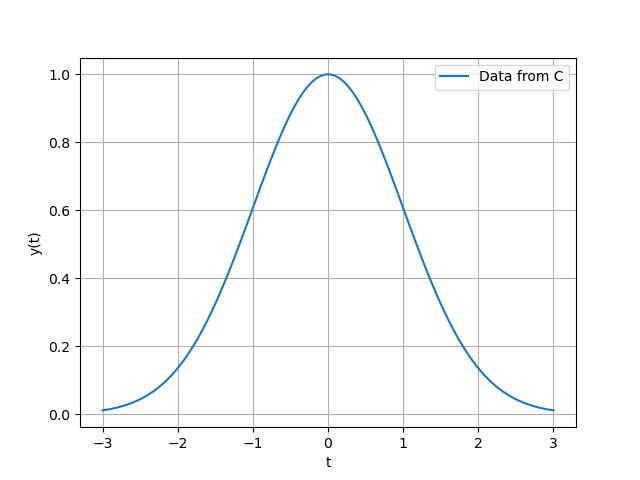
\includegraphics[width=\columnwidth]{2023/CE/30/figs/graph_of_y(t).png}
    \caption{Graph of y(t)}
    \label{fig:Graph1_gate_CE_30}
    \end{figure}


\pagebreak

\end{enumerate}
